\documentclass[residuals.tex]{subfiles}
\begin{document}
\Large
\section{Cook's Distance}	
	\begin{itemize}
		\item In statistics, Cook's distance or Cook's D is a commonly used estimate of the influence of a data point when performing least squares regression analysis.
		
		\item Cook's distance is useful for identifying outliers in the X values (observations for predictor variables). It also shows the influence of each observation on the fitted response values. 
		
		\item 
		Cook's distance is the scaled change in fitted values. Each resulting element in a diagnostic calculation is the normalized change in the vector of coefficients due to the deletion of an observation. 
		
		\item In a practical ordinary least squares analysis, Cook's distance can be used in several ways: to indicate data points that are particularly worth checking for validity; to indicate regions of the design space where it would be good to be able to obtain more data points. 
		\item 
		It is named after the American statistician R. Dennis Cook, who introduced the concept in 1977.
		
		\item 
		Cook's distance measures the effect of deleting a given observation. Data points with large residuals (outliers) and/or high leverage may distort the outcome and accuracy of a regression. 
		
		\item Points with a large Cook's distance are considered to merit closer examination in the analysis. 
		
		\item Influential cases are not usually a problem when their removal from the dataset would leave the parameter estimates essentially unchanged: the ones we worry about are those whose presence really does change the results. 
		\item 	Cook's D is a good measure of the influence of an observation and is proportional to the sum of the squared differences between predictions made with all observations in the analysis and predictions made leaving out the observation in question. If the predictions are the same with or without the observation in question, then the observation has no influence on the regression model. If the predictions differ greatly when the observation is not included in the analysis, then the observation is influential.
	\end{itemize}
\newpage
\subsection*{Cook's Distance Formula}
It is calculated as:
\[D_i = \frac{ \sum_{j=1}^n (\hat Y_j\ - \hat Y_{j(i)})^2 }{p \ \mathrm{MSE}},
\]

where:
\begin{itemize}
	\item $\hat Y_j$ \, is the prediction from the full regression model for observation j;
	\item $\hat Y_{j(i)}$\, is the prediction for observation j from a refitted regression model in which observation i has been omitted;
	\item $p$ is the number of fitted parameters in the model;
	\item $\mathrm{MSE} $ \, is the mean square error of the regression model.
	
\end{itemize}
\newpage
For the case of simple linear regression, the following are the algebraically equivalent expressions 
\[D_i = \frac{e_i^2}{p \ \mathrm{MSE}}\left[\frac{h_{ii}}{(1-h_{ii})^2}\right],
\]

\[
D_i = \frac{ (\hat \beta - \hat {\beta}^{(-i)})^T(X^TX)(\hat \beta - \hat {\beta}^{(-i)}) } {(1+p)s^2},
\]

where:
\begin{itemize}
\item $h_{ii} \,$ is the leverage, i.e., the i-th diagonal element of the hat matrix  \[\mathbf{X}\left(\mathbf{X}^T\mathbf{X}\right)^{-1}\mathbf{X}^T\]
\item $e_i$ \, is the residual (i.e., the difference between the observed value and the value fitted by the proposed model).
\end{itemize}


%============================================================================================================%
\bigskip
	

% (Cohen, Cohen, West \& Aiken, 2003).
	%==================================================================%
	\newpage
\subsection*{ \texttt{R} code for computing Cook's Distance}	
\begin{framed}
	\begin{verbatim}
	attach(mtcars)
	fit = lm(mpg ~ cyl + wt )
	cooks.distance(fit)
	plot(cooks.distance(fit),type="b",pch=18,col="red")
	
	N = 32
	k = 2
	cutoff = 4/ (N-k-1)
	abline(h=cutoff,lty=2)
	\end{verbatim}
\end{framed}

\begin{figure}[h!]
\centering
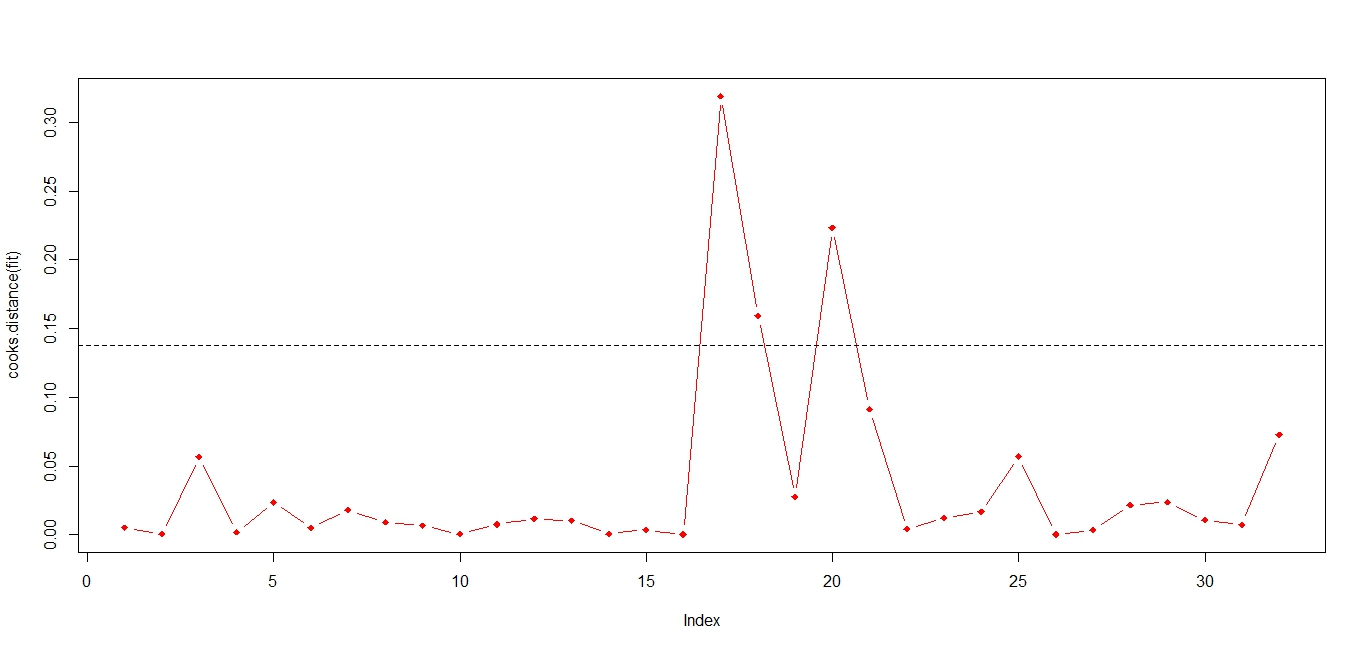
\includegraphics[width=0.9\linewidth]{cooksplot}
\caption{}
\label{fig:cooksplot}
\end{figure}


\newpage


\subsection{Interpreting Cook's Distance}
\begin{quote}
A common rule of thumb is that an observation with a value of Cook's D over 1.0 has too much influence. As with all rules of thumb, this rule should be applied judiciously and not thoughtlessly. (John Fox)\\ \textit{(1991). Regression Diagnostics: An Introduction. Sage Publications.}
\end{quote}
% Interpretation
% http://stats.stackexchange.com/questions/22161/how-to-read-cooks-distance-plots%
\bigskip
\begin{itemize}
\item Some texts tell you that points for which Cook's distance is higher than 1 are to be considered as influential. 
\item Other texts give you a threshold of $4/N$ or \[ {4  \over (N-k-1)} ,\] where N is the number of observations and k the number of explanatory variables. 
\item The \texttt{R} help file advises that an observation with Cook's distance larger than three times the mean Cook's distance might be an outlier. .

\item John Fox (mentioned above), in his booklet on regression diagnostics is rather cautious when it comes to giving numerical thresholds. He advises the use of graphics and to examine in closer details the points with "values of D that are substantially larger than the rest". According to Fox, thresholds should just be used to enhance graphical displays.
\end{itemize}



\newpage	

\subsubsection*{Remark}	

\begin{itemize}
\item Cook's distance refers to how far, on average, predicted y-values will move if the observation in question is dropped from the data set. 
\item \textbf{DFBETA} :  \textit{DFBETA} refers to how much a parameter estimate changes if the observation in question is dropped from the data set.

\item  \textit{Note that with k covariates, there will be k+1 DFBETAs (the intercept, $\beta_0$, and $\beta_1$ for each covariate).}
\item  Cook's distance is arguably more important if you are doing predictive modeling, whereas \textit{DFBETA} is more important in explanatory modeling.
\item \textbf{DFFITS}: Although the raw values resulting from the equations are different, Cook's distance and \textit{DFFITS} are conceptually identical and there is a closed-form formula to convert one value to the other.
\end{itemize}



%Detecting highly influential observations[edit]
%There are different opinions regarding what cut-off values to use for spotting highly influential points. A simple operational guideline of D_i>1 has been suggested.[2] Others have indicated that D_i>4/n, where n is the number of observations, might be used.[3]
%A conservative approach relies on the fact that Cook's distance has the form W/p, where W is formally identical to the Wald statistic that one uses for testing that H_0:\beta_i=\beta_0 using some \hat{\beta}_{[-i]}.[citation needed] Recalling that W/p has an F_{p,n-p} distribution (with p and n-p degrees of freedom), we see that Cook's distance is equivalent to the F statistic for testing this hypothesis, and we can thus use F_{p,n-p, 1-\alpha} as a threshold.
%Interpretation[edit]
%Specifically D_i can be interpreted as the distance one's estimates move within the confidence ellipsoid that represents a region of plausible values for the parameters.[clarification needed] This is shown by an alternative but equivalent representation of Cook's distance in terms of changes to the estimates of the regression parameters between the cases where the particular observation is either included or excluded from the regression analysis.




\end{document}
